%*****************************************
\chapter{Working With Data}\label{ch07:data}
%*****************************************

Lorem ipsum dolor sit amet, consectetuer adipiscing elit. Aenean commodo ligula eget dolor. Aenean massa. Cum sociis natoque penatibus et magnis dis 

\section{Importing Data}

\begin{center}
	\begin{objbox}{Learning Objectives}
		\begin{itemize}
			\setlength{\itemsep}{0pt}
			\setlength{\parskip}{0pt}
			\setlength{\parsep}{0pt}
			
			\item Data can be imported from many sources, including the web, databases, or local files.
			\item Tools on the \fmtRibbonTab{Data} tab of the ribbon make it easy to import data.

		\end{itemize}
	\end{objbox}
\end{center}

To use Excel's powerful tools for analysis, data must first be imported into a spreadsheet. Data can be imported from many sources but two common ones are from the web and from a datafile located on the local computer. Data is very often posted on the web for researchers to use in their projects. The United States federal government, for example, has more than $ 200,000 $ datasets freely available in fields like taxes, crime, trade, education, and dozens of other topics\footnote{See \url{https://www.data.gov/}}. Sometimes, that data can be imported directly into Excel but more often it must be downloaded to a local computer and then imported into Excel from that file. This section demonstrates both of those procedures.

\subsection{Import From the Web}

Data in a table on a website can be imported directly into an Excel workbook. Follow these steps to import data from a website.

\begin{enumerate}
	\item Open a new file with a blank workbook.
	\item Save the file as \fmtWorkbookName{WebData.xlsx}.
	\item Click \fmtRibbonGroup{Get External Data} in the \fmtRibbonTab{Data} tab of the ribbon.
	\item Click \fmtPopupButton{From Web} in the popup menu, as shown in Figure \ref{07:fig01}.
\end{enumerate}

\begin{figure}[H]
	\centering
	\includegraphics[width=\maxwidth{.95\linewidth}]{gfx/ch07_fig01}
	\caption{Import From Web Menu}
	\label{07:fig01}
\end{figure}

For this exercise, a page on Wikipedia that has several data tables will be used. The URL is: \url{https://en.wikipedia.org/wiki/Largest_airlines_in_the_world}

\begin{enumerate}[resume]
	\item Enter the URL in the \fmtPopupBox{From Web} popup.
	\item Press \fmtPopupButton{GO}
	\item Excel will access the website and open the \fmtPopupBox{Navigator} window, as shown in Figure \ref{07:fig02}.
\end{enumerate}

\begin{figure}[H]
	\centering
	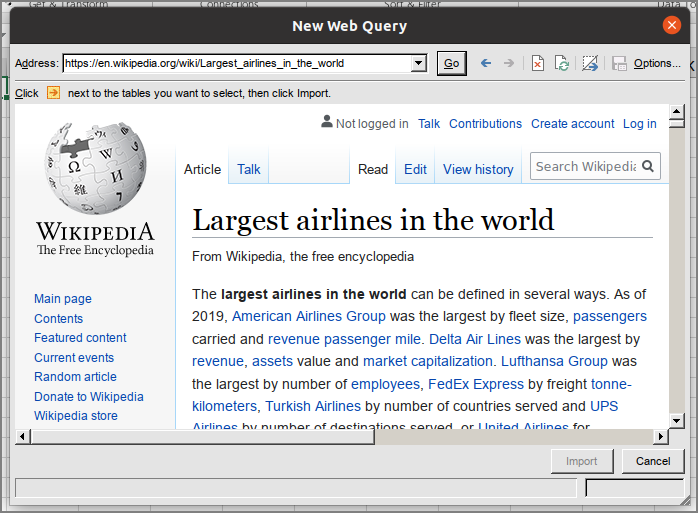
\includegraphics[width=\maxwidth{.95\linewidth}]{gfx/ch07_fig02}
	\caption{From Web URL Window}
	\label{07:fig02}
\end{figure}

%\begin{figure}[H]
%	\centering
%	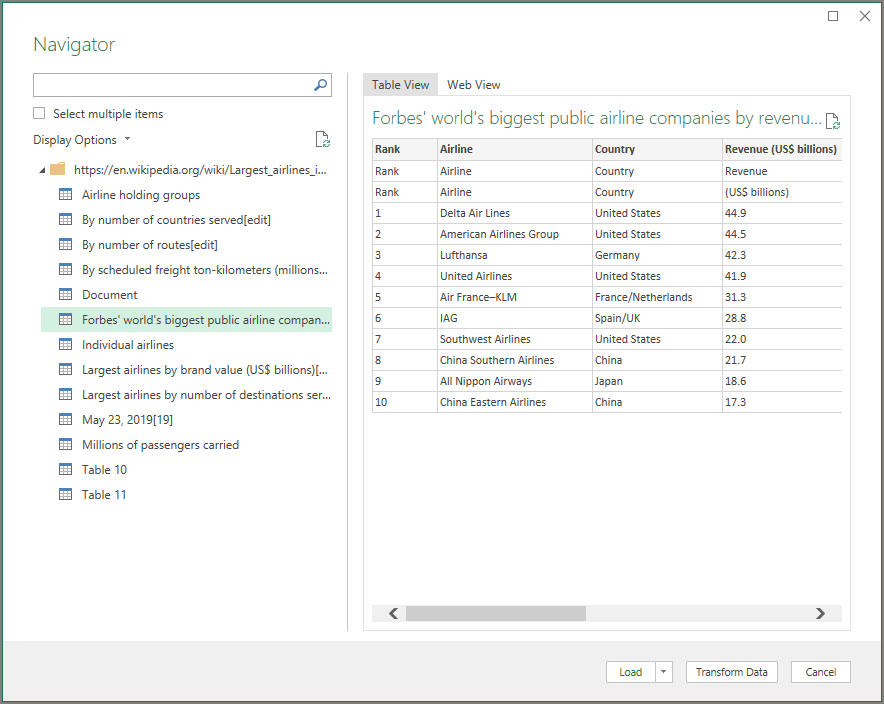
\includegraphics[width=\maxwidth{.95\linewidth}]{gfx/ch07_fig03}
%	\caption{Navigator Window}
%	\label{07:fig03}
%\end{figure}


\begin{enumerate}[resume]
	\item Scroll down the displayed page until the desired table is visible. Notice a small arrow icon to the left of the table. Click that icon to mark the table for downloading, then click the \fmtPopupButton{Import} button. Figure \ref{07:fig04} shows the data table loaded into Excel.
\end{enumerate}

\begin{figure}[H]
	\centering
	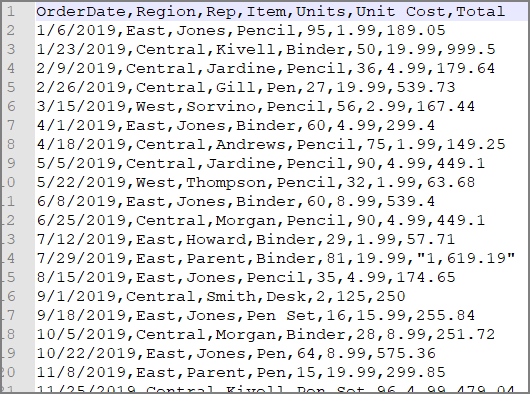
\includegraphics[width=\maxwidth{.95\linewidth}]{gfx/ch07_fig04}
	\caption{Imported Data Table}
	\label{07:fig04}
\end{figure}

Notice that the data is imported into a new worksheet. Excel now displays a \fmtPopupBox{Queries \& Connections} box on the right side of the screen. That box lists the Web queries that were used to import data tables. Since there has only been one query then only one line appears in this box, but if more queries are run they will also be listed here. 

\begin{enumerate}[resume]
	\item Close the \fmtPopupBox{Queries \& Connections} box by clicking the \fmtPopupButton{X} in the top right corner of the box.
\end{enumerate}

A data table is imported into Excel as a table, so tools like filtering, sorting, and slicing the data are readily available. As with any Excel table, this data table can be recolored and formatted as desired. Those skills, though, are taught elsewhere in this class and are not further covered here.

\subsection{Import From Data File}

\textit{Data file: CH7-Data}

It is common for web data to be downloaded via a data file. Those data files are, typically, in a \textit{.CSV} format. This is a simple text file and can be opened with a program no more complicated than Notepad; but they are typically opened with Excel or some other data analysis tool. Figure \ref{07:fig05} shows the first few lines of the sales data file used in this lesson opened in Notepad.

\begin{figure}[H]
	\centering
	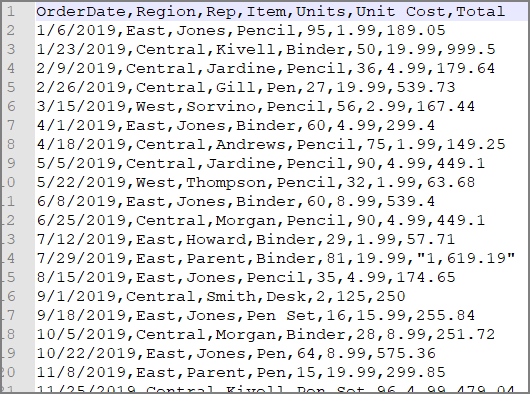
\includegraphics[width=\maxwidth{.95\linewidth}]{gfx/ch07_fig05}
	\caption{CSV File}
	\label{07:fig05}
\end{figure}

Complete the following steps to load a \textit{.CSV} file into Excel.

\begin{enumerate}
	\item Click \fmtRibbonButton{Get External Data} in the \fmtRibbonTab{Data} tab of the ribbon.
	\item Click \fmtPopupButton{From Text}. Figure \ref{07:fig06} illustrates this button.
\end{enumerate}

\begin{figure}[H]
	\centering
	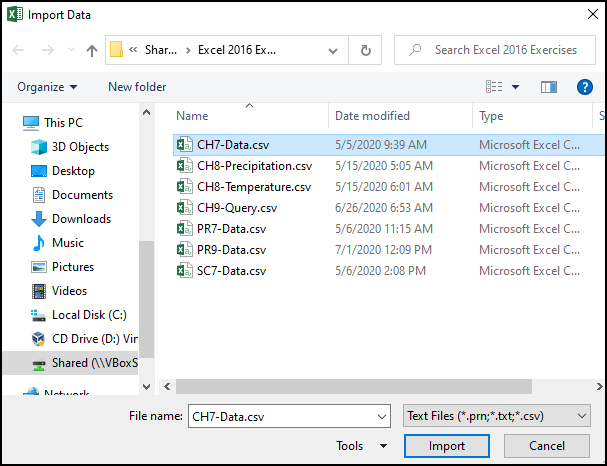
\includegraphics[width=\maxwidth{.95\linewidth}]{gfx/ch07_fig06}
	\caption{Import CSV File}
	\label{07:fig06}
\end{figure}

\begin{enumerate}
	\item Navigate to the data file.
	\item Click the file name and then \fmtPopupButton{Import}. Figure \ref{07:fig07} shows the \fmtPopupBox{Import Text File} dialog box.
\end{enumerate}

\begin{figure}[H]
	\centering
	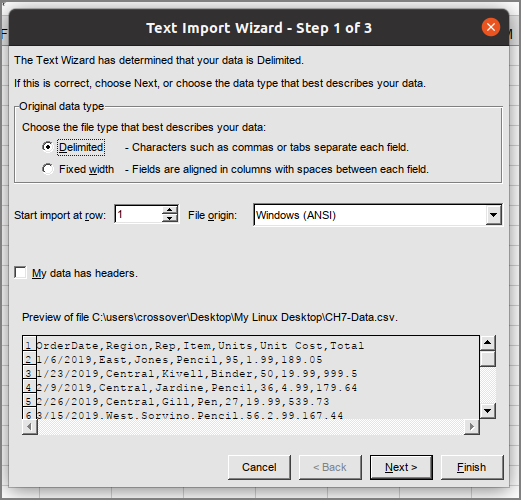
\includegraphics[width=\maxwidth{.95\linewidth}]{gfx/ch07_fig07}
	\caption{Selecting the CSV file}
	\label{07:fig07}
\end{figure}

\begin{enumerate}
	\item Excel will begin to import the .CSV data. Excel starts a wizard that contains its ``best guess'' about the type of data in the file, as illustrated in Figure \ref{07:fig08}.
\end{enumerate}

\begin{figure}[H]
	\centering
	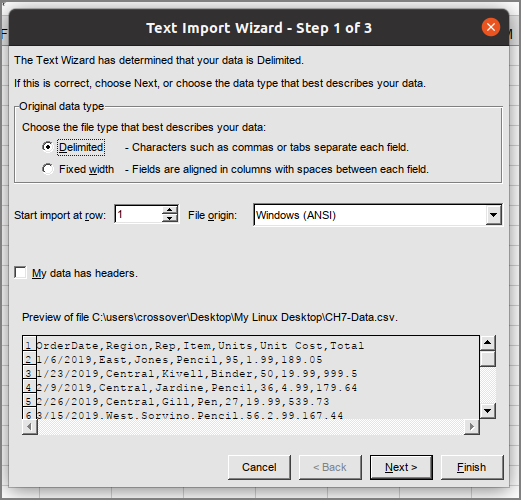
\includegraphics[width=\maxwidth{.95\linewidth}]{gfx/ch07_fig08}
	\caption{Step One of the Text Import Wizard}
	\label{07:fig08}
\end{figure}

\begin{enumerate}
	\item The sample text contained in the box at the bottom of Figure \ref{07:fig08} looks correct, so Excel has correctly determined that the CSV file contains delimited text using Windows format. Click \fmtPopupButton{Next}.
	\item For this data, it is appropriate to begin the import at row 1, but that can be changed if there are several explanatory lines at the top of the file.
	\item Click the \fmtPopupButton{My data has headers} checkbox since the first line of the data contains column headers.
	\item Click \fmtPopupButton{Next}.
	\item Figure \ref{07:fig09} shows that Excel is now guessing that a tab is being used to separate the data columns, but that is not correct. Click the checkbox for \fmtPopupButton{Comma} and notice that the sample data in the box at the bottom of the screen separates into columns.
\end{enumerate}

\begin{figure}[H]
	\centering
	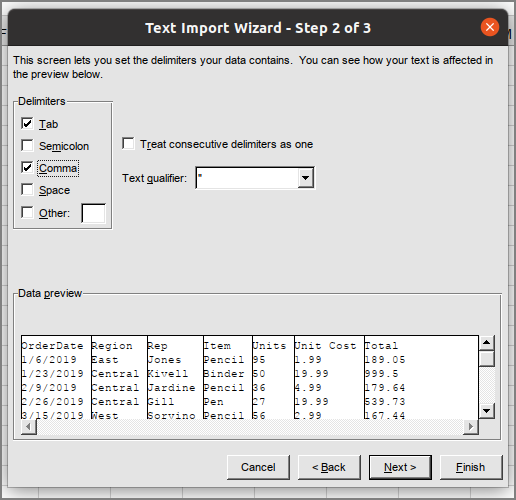
\includegraphics[width=\maxwidth{.95\linewidth}]{gfx/ch07_fig09}
	\caption{Defining Delimiters in the Data Import Wizard}
	\label{07:fig09}
\end{figure}

\begin{enumerate}
	\item Step three of the data import wizard permits users to identify the type of data contained in each column. For this import, click on column one to highlight it and then click on the \fmtPopupButton{Date:} button to define this column as dates. The \textit{MDY} date format option is correct.
	\item Click \fmtPopupButton{Finish} to complete the wizard.
	\item Excel now asks if the data should be loaded into the existing worksheet or create a new worksheet, as illustrated in Figure \ref{07:fig10}.
	\item For this exercise, load the data into cell \fmtCellLocation{A1} in the existing worksheet.
\end{enumerate}

\begin{figure}[H]
	\centering
	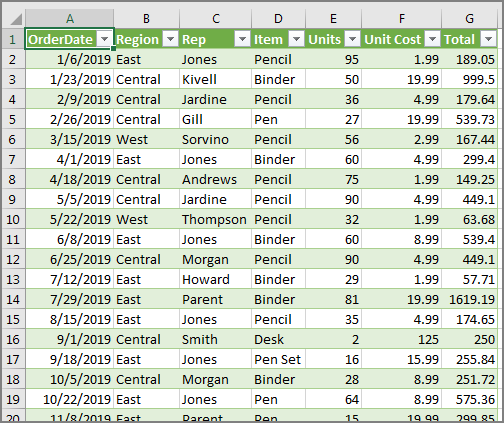
\includegraphics[width=\maxwidth{.95\linewidth}]{gfx/ch07_fig10}
	\caption{Loading the Data}
	\label{07:fig10}
\end{figure}

Figure \ref{07:fig11} shows the first few lines of the worksheet with the imported data.

\begin{figure}[H]
	\centering
	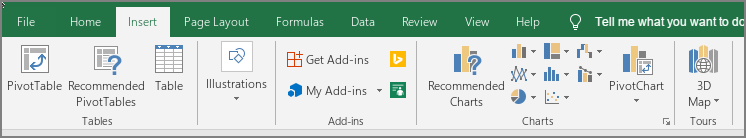
\includegraphics[width=\maxwidth{.95\linewidth}]{gfx/ch07_fig11}
	\caption{The Worksheet With Imported Data}
	\label{07:fig11}
\end{figure}

\begin{enumerate}[resume]
	\item Rename the worksheet to \fmtWorksheetName{Sales Data}.
	\item Save the workbook.
\end{enumerate}

\begin{center}
	\begin{tkwbox}{Key Take-Aways}
		\textbf{Importing Data}
		\\
		\begin{itemize}
			\setlength{\itemsep}{0pt}
			\setlength{\parskip}{0pt}
			\setlength{\parsep}{0pt}
			
			\item Data can be imported from tables found on websites using \fmtRibbonButton{From Web} on the \fmtRibbonGroup{Get \& Transform} group on the \fmtRibbonTab{Data} tab on the ribbon.
			\item Data can be imported from CSV files downloaded from websites using \fmtRibbonButton{From Text} on the \fmtRibbonGroup{Get External Data} group on the \fmtRibbonTab{Data} tab on the ribbon.
			
		\end{itemize}
	\end{tkwbox}
\end{center}

\section{Pivot Tables}

\begin{center}
	\begin{objbox}{Learning Objectives}
		\begin{itemize}
			\setlength{\itemsep}{0pt}
			\setlength{\parskip}{0pt}
			\setlength{\parsep}{0pt}

			\item Create a pivot table.
			\item Manipulate a pivot table to change the information displayed.
			
		\end{itemize}
	\end{objbox}
\end{center}

Pivot tables dynamically summarize data and are a favorite tool for analysts since they are highly customizable and very powerful. Pivot tables are sometimes called contingency tables or crosstabs and are frequently seen in reports where tabular data is presented like the number of voters who support a proposition broken down by party affiliation, race, or other factors. For this exercise, the data from the sales data imported above is analyzed.

\begin{enumerate}
	\item Click in cell \fmtCellLocation{A1} in the \fmtWorksheetName{Sales Data} worksheet.
	\item Click \fmtRibbonButton{PivotTable} in the \fmtRibbonGroup{Tables} group on the \fmtRibbonTab{Insert} tab of the ribbon.
	\item In the \fmtPopupBox{Create PivotTable} popup, ensure that Excel automatically selected \$A\$1:\$G\$44, which is all the data on the worksheet. Also, ensure \fmtPopupButton{New Worksheet} is selected as the location of the new PivotTable. Figure \ref{07:fig12} illustrates the PivotTable wizard.
	\item Click \fmtPopupButton{OK}.
\end{enumerate}

\begin{figure}[H]
	\centering
	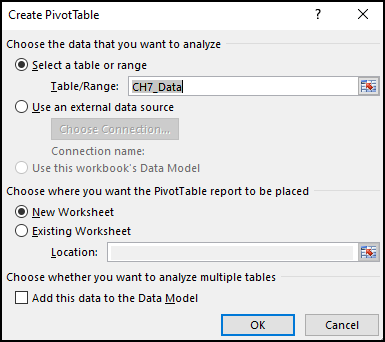
\includegraphics[width=\maxwidth{.95\linewidth}]{gfx/ch07_fig12}
	\caption{Create PivotTable Wizard}
	\label{07:fig12}
\end{figure}


\begin{enumerate}[resume]
	\item A pivot table is created on a new worksheet. Rename that sheet \fmtWorksheetName{Sales Pivot}.
	\item Move the \fmtWorksheetName{Sales Pivot} worksheet to the right of \fmtWorksheetName{Sales Data}.
	\item A blank pivot table has six areas of interest for this lesson, as shown in Figure \ref{07:fig13}.

	\begin{itemize}
		\item \textbf{A}. The Pivot Table will appear in the large area on the left (it is blank in the illustration).
		\item \textbf{B}. The Field List contains the names of all the fields (columns) in the data set.
		\item \textbf{C}. Filters is where the pivot table data can be filtered.
		\item \textbf{D}. Column Labels define the columns found in the pivot table.
		\item \textbf{E}. Row Labels define the rows found in the pivot table.
		\item \textbf{F}. Values define the numeric data calculated in the pivot table.
	\end{itemize}
\end{enumerate}

\begin{figure}[H]
	\centering
	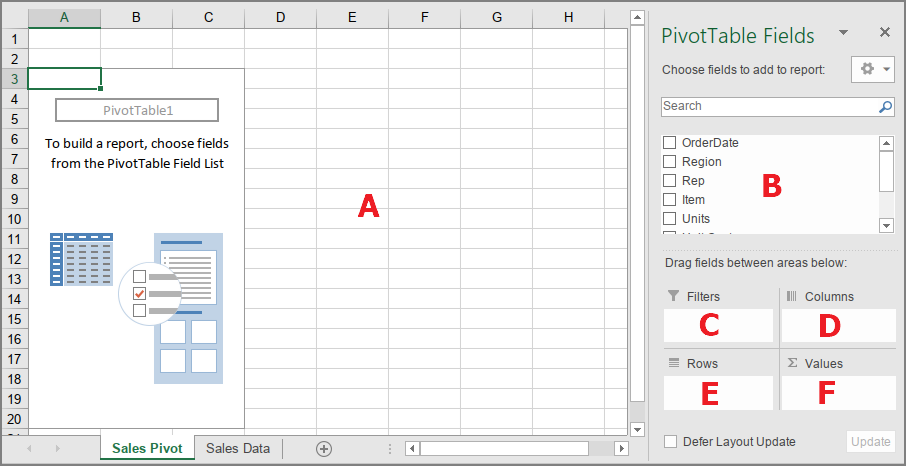
\includegraphics[width=\maxwidth{.95\linewidth}]{gfx/ch07_fig13}
	\caption{Pivot Table Areas}
	\label{07:fig13}
\end{figure}

\begin{enumerate}[resume]
	\item Check \textit{Region} in the Field List. By default, Excel places that item in the Row Labels area since it contains text labels. (Note: \textit{Region} can also be dragged to the Row Labels area.)
	\item Check \textit{Item} in the Field List. By default, Excel places Item in the Row Labels area since it contains text labels. (Note: \textit{Item} can also be dragged to the Row Labels area.)
	\item Check \textit{Units} in the Field List. By default, Excel places that Units in the Values area since it contains numbers (notice that Excel automatically creates a sum of Units, but that can be changed to average, max, min, or other statistical values). 
	\item The pivot table now shows how many units of each type of product was sold in each area. There is also a Grand Total at the bottom of the pivot table. With just a few clicks of the mouse, Excel has created a useful decision-making chart for managers.
	\item Click and drag \textit{Item} from the Row Labels area to the Column Labels area. (Note, this can also be done by clicking the down-arrow for \textit{Item} and selecting \fmtPopupButton{Move to Column Labels}.) The same data is still being displayed, but it has been rearranged to make it easier to compare regions.
	\item Uncheck \textit{Units} in the Field List. This removes it from the pivot table and leaves only labels with no numbers.
	\item Check \textit{Total} in the Field List. By default, Excel places that item in the Values area since it contains numbers (notice Excel automatically creates a sum of Total). The table now reports the total value of all sales by region and item.
	\item Change the value displayed to average rather than sum.
	
	\begin{enumerate}
		\item Click the down arrow in \textit{Sum of Total} in the Values area. 
		\item Select \fmtPopupButton{Value Field Settings}.
		\item Select \fmtPopupButton{Average} in the popup.
		\item Click \fmtPopupButton{OK}.
		\item The PivotTable is instantly changed to display the average sales by region and item.
	\end{enumerate}

	\item The average is displayed to seven decimal places. Since this is money, it would be best to round the averages to two decimal places.

	\begin{enumerate}
		\item Click the down arrow in \textit{Average of Total} in the Values area. 
		\item Select \fmtPopupButton{Value Field Settings}.
		\item Click the \fmtPopupButton{Number Format} button at the bottom left corner of the \fmtPopupBox{Value Field Settings} popup.
		\item Choose \fmtPopupButton{Currency} and accept the default settings.
		\item Click \fmtPopupButton{OK}.
		\item Click \fmtPopupButton{OK}.
		\item The pivot table is instantly changed to display currency.
	\end{enumerate}
	
	\item Uncheck all fields to remove them from the pivot table.
	\item Check \textit{OrderDate} in the Field List. By default, Excel places that item in the pivot table Row Labels area since it contains dates. Notice that Excel automatically expands the dates into years, quarters, and dates.
	\item Drag \textit{Total} from the Field List to Values. The pivot table now shows the total sales by date. Clicking the plus sign beside the years and quarters permits users to drill down to specific quarters and months of interest.
	\item Drag \textit{Region} from the Field List to Columns. This creates columns for each region in the pivot table so now management can find sales by month and region.
	\item To filter the data, click the down arrow to the right of the \textit{Column Labels} header. Uncheck all regions except \textit{East} and notice how the pivot table is updated to include only the East region.
	\item While managers normally like having dates grouped by month/quarter/year, that can be easily modified. Click \textit{2019} in the pivot table so only that one cell is selected. Click the \fmtRibbonButton{Group Field} button in the \fmtRibbonGroup{Group} group in the \fmtRibbonTab{Analyze} tab. 
	\item The \fmtPopupBox{Grouping} popup box appears so the start/end dates for the data can be specified. For this excercise, leave the dates at their default (the entire year), but click \textit{months} so it is no longer highlighted then click \fmtPopupButton{OK}. This will remove the \textit{Months} drill down capability and only show years and quarters in the pivot table. By using this option, details can be removed from the pivot table so trends may become more visible.
	\item Drag \textit{Rep} from the Field List to the Filters area. Notice that the pivot table now has a selector in cell \fmtCellLocation{B1} so a specific representative (or group of representatives) can be used to filter data on the pivot table. Click the down arrow for the \textit{Rep} filter and select \fmtPopupButton{Andrews}. Notice that the pivot table is instantly updated to include only Andrews' sales data.
	\item This pivot table will be used to create a pivot chart in the next section; however, the filter is not needed. Uncheck \textit{Rep} in the Field List to remove that from the filter area.
\end{enumerate}

\begin{center}
	\begin{tkwbox}{Key Take-Aways}
		\textbf{Pivot Tables}
		\\
		\begin{itemize}
			\setlength{\itemsep}{0pt}
			\setlength{\parskip}{0pt}
			\setlength{\parsep}{0pt}
			
			\item Pivot tables are a very powerful analysis tool that are easy to create and use.
			
		\end{itemize}
	\end{tkwbox}
\end{center}

\section{Pivot Charts}

\begin{center}
	\begin{objbox}{Learning Objectives}
		\begin{itemize}
			\setlength{\itemsep}{0pt}
			\setlength{\parskip}{0pt}
			\setlength{\parsep}{0pt}
			
			\item one
			
		\end{itemize}
	\end{objbox}
\end{center}

One of the strengths of creating a PivotTable is to use that table to create a chart. Follow these directions to explore the power of this feature.

\begin{enumerate}
	\item Open Advanced\_Exercises.xlsx.
	\item Select the Inventory worksheet. 
	\item Click in any cell that contains data, like A2.
	\item Click Insert $\rightarrow$ Tables $\rightarrow$ Pivot Table.
	\item In the Create PivotTable popup, ensure that Excel automatically selected A1:I51, which is all the data on the worksheet. Also, ensure “New Worksheet” is selected as the location of the new PivotTable.
	\item A pivot table is created on a new worksheet. Rename that sheet “Inventory Chart.”
	\item Check the Distributor item in the Field List. By default, Excel places that item in the pivot table Row Labels area since it contains text labels.
	\item Check the Genre item in the Field List. By default, Excel places that item in the pivot table Row Labels area since it contains text labels.
	\item Check the On Hand item in the Field List. By default, Excel places that item in the pivot table Values area since it contains numbers (notice that Excel automatically creates a sum of On Hand). The pivot table now shows how many movies are in the inventory for each genre by each distributor.
	\item Click and drag Genre from the Row Labels area to the Column Labels area. (Note, this can also be done by clicking the down-arrow for Genre and selecting “Move to Column Labels”.)
	\item Click Insert $\rightarrow$  Charts $\rightarrow$ Pivot Chart.
	\item Select the default “Clustered Column” chart. The chart that is created is linked to the pivot table so any changes in that table will be reflected in the chart.
	\item Uncheck the On Hand item in the Field list. 
	\item Check the Total item in the Field list. By default, Excel places that item in the Values area since it contains numbers (notice Excel automatically creates a sum of Total). The table now reports the total value of all movies in the inventory, by distributor and genre.
	\item On the pivot chart, click the down arrow on the Genre legend title (illustrated on the right) to open a filter. Uncheck everything except action, drama, and sci-fi.
	\item Continue to explore this powerful feature by changing the PivotTable elements and observing the change to the chart.
\end{enumerate}

\begin{center}
	\begin{tkwbox}{Key Take-Aways}
		\textbf{Pivot Charts}
		\\
		\begin{itemize}
			\setlength{\itemsep}{0pt}
			\setlength{\parskip}{0pt}
			\setlength{\parsep}{0pt}
			
			\item one
			
		\end{itemize}
	\end{tkwbox}
\end{center}

\section{Using the Statistics Ribbon Tab}

\begin{center}
	\begin{objbox}{Learning Objectives}
		\begin{itemize}
			\setlength{\itemsep}{0pt}
			\setlength{\parskip}{0pt}
			\setlength{\parsep}{0pt}
			
			\item one
			
		\end{itemize}
	\end{objbox}
\end{center}

Lorem ipsum dolor sit amet, consectetuer adipiscing elit. Aenean commodo ligula eget dolor. Aenean massa. Cum sociis natoque penatibus et magnis dis 

\begin{center}
	\begin{tkwbox}{Key Take-Aways}
		\textbf{Using the Statistics Ribbon Tab}
		\\
		\begin{itemize}
			\setlength{\itemsep}{0pt}
			\setlength{\parskip}{0pt}
			\setlength{\parsep}{0pt}
			
			\item one
			
		\end{itemize}
	\end{tkwbox}
\end{center}

\section{What-if Analysis}

\begin{center}
	\begin{objbox}{Learning Objectives}
		\begin{itemize}
			\setlength{\itemsep}{0pt}
			\setlength{\parskip}{0pt}
			\setlength{\parsep}{0pt}
			
			\item one
			
		\end{itemize}
	\end{objbox}
\end{center}

One of the most important uses for a computerized spreadsheet like Excel over a paper-and-pencil system is the ability to quickly test various business parameters to forecast profits. Two forecasting techniques are commonly used and the best way to learn about them is to work through examples. 

\subsection{Data Table}

A data table is the simplest forecasting technique. Excel can fill the cells of a data table with values that are the result of repeatedly applying a formula to a range of data. As an example, imagine that Riley was buying a new car that cost \$35,000. The dealership offered financing at 6\% but the term (length of the loan) was flexible. Riley wanted to know what term to choose to get the maximum payment that is still under \$1000.

\begin{enumerate}
	\item Open Advanced\_Exercises.xlsx.
	\item Select the One Var Data Table worksheet.
	\item Notice that some information has already been started, including the loan amount (cell B3), interest rate (cell B4), and term (cell B5).
	\item Enter this formula to calculate the size of a monthly payment in cell B6: =PMT(B4/12,B5,B3) (Note: this is an Excel formula that is used to calculate payments.)
	\item In cell E3 enter: =B6.
	\item In cell D4:D11 enter 12, 18, 24, 30, 36, 42, 48, 54, 60 (using autofill may make this quicker).
	\item Select D3:E11
	\item Click Data $\rightarrow$ Forecast $\rightarrow$ What-if Analysis $\rightarrow$ Data Table.
	\item In the Data Table properties, enter B5 for Column input cell (leave the Row input cell blank since this data table has only one column with no rows). Excel will substitute values from D4:D12 into cell B5 one at a time and find the result using the formula in E3.
	\item Click OK.
\end{enumerate}

Riley should choose a term of 42 months since that creates the largest payment that is less than \$1000. Note: the payments are represented as negative numbers because they represent money that is leaving Riley’s bank account.

In the one-variable example above only one variable, term, was changed to determine its impact on the payment. Excel can also build a data table that reflects changing two variables. Morgan is investing some savings in a fund that has an annual percentage rate of 5\%. Morgan can invest anywhere from \$1000 to \$10000 for any number of years from 2 to 7 and is interested to see how that investment will grow.

\begin{enumerate}
	\item Open Advanced\_Exercises.xlsx.
	\item Select the Two Var Data Table worksheet.
	\item Notice that some information has already been started, including the initial investment (cell B3), annual percentage rate (cell B4), number of compounding periods per year (B5), and the number of years (cell B6).
	\item Enter this formula to calculate the future value of the investment in cell B7: =FV(B4/B5,B6*B5,,-B3). (This is an Excel formula that is used to calculate the future value of an investment. Note the negative sign before the last term.)
	\item In cell D3 enter: =B7.
	\item In cell D4:D13 enter 1000, 2000, 3000, 4000, 5000, 6000, 7000, 8000, 9000, 10000.
	\item In cell E3:J3 enter 2, 3, 4, 5, 6, 7.
	\item Select D3:J13.
	\item Click Data $\rightarrow$ Forecast $\rightarrow$ What-if Analysis $\rightarrow$ Data Table.
	\item In the Data Table properties, enter B6 for Row input cell and B3 for Column input cell.
	\item Click OK.
\end{enumerate}

\subsection{Goal Seek}

Often, business owners know the goal they seek, and they want Excel to determine what parameter to set to achieve that goal. The following exercise demonstrates goal seeking. Imagine that a business owner wants to know how much money to take in (“receipts”) to generate \$100,000 in profit.

\begin{enumerate}
	\item Open Advanced\_Exercises.xlsx.
	\item Select the Goal Seek worksheet.
	\item This worksheet already includes some data: the company receipts (B2), the cost of food as a percentage of receipts (B3), the overhead as a percentage of receipts (B4), and a place for the net profit calculation (B5).
	\item Enter this formula in B5: =B2-((B2*B3)+(B2*B4)).
	\item Click Data $\rightarrow$ Forecast $\rightarrow$ What-if Analysis $\rightarrow$ Goal Seek.
	\item For Set cell enter \$B\$5, for To value enter 100,000, for By changing cell enter \$B\$2.
	\item Click OK.
\end{enumerate}

The data on the worksheet will adjust to fit the requirement. Clicking OK on the Goal Seek Status popup will change the worksheet, clicking Cancel will revert the worksheet back to its original values.
Try using Goal Seek to change the overhead percentage to yield a profit of \$35,000 with receipts of \$100,000. 

\begin{center}
	\begin{tkwbox}{Key Take-Aways}
		\textbf{What-if Analysis}
		\\
		\begin{itemize}
			\setlength{\itemsep}{0pt}
			\setlength{\parskip}{0pt}
			\setlength{\parsep}{0pt}
			
			\item one
			
		\end{itemize}
	\end{tkwbox}
\end{center}

\section{Using Excel Macros}

\begin{center}
	\begin{objbox}{Learning Objectives}
		\begin{itemize}
			\setlength{\itemsep}{0pt}
			\setlength{\parskip}{0pt}
			\setlength{\parsep}{0pt}
			
			\item one
			
		\end{itemize}
	\end{objbox}
\end{center}

The View $\rightarrow$ Macros $\rightarrow$ Macros button allows users to automate repetitive tasks. The top part of the button will open the View Macros dialog box and the bottom half reveals options for macros. There is also a Record Macro button on the status bar at the bottom left corner of the worksheet. 
Follow these steps to create a very simple macro.


\begin{center}
	\begin{tkwbox}{Key Take-Aways}
		\textbf{Using Excel Macros}
		\\
		\begin{itemize}
			\setlength{\itemsep}{0pt}
			\setlength{\parskip}{0pt}
			\setlength{\parsep}{0pt}
			
			\item one
			
		\end{itemize}
	\end{tkwbox}
\end{center}

\begin{enumerate}
	\item Open a new blank workbook. (Note: the macro is placed in a new workbook so it does not accidentally interfere with the exercises in this lesson’s workbook.) 
	\item Click A1 to select that cell.
	\item Click View $\rightarrow$ Macros $\rightarrow$ Macros (be sure to click the small arrow at the bottom of the “Macros” button).
	\item Select Use Relative References.
	\item Select Record Macro.
	\item Call the macro MyName.
	\item Click in the “Shortcut Key” box and type Shift+Q.
	\item Store the macro in this workbook.
	\item Enter this description: Inserts my name. 
	\item Click OK.
	\item Type your first and last name and press Enter.
	\item Click View $\rightarrow$ Macros $\rightarrow$ Macros (be sure to click the small arrow at the bottom of the “Macros” button).
	\item Select Stop Recording.
\end{enumerate}

Select another cell on the worksheet and press Ctrl-Shift+Q. In step 4, relative references were activated for the macro. If that had not been done, then the name would have always been created in cell A1 (the original cell) instead of the current cell.

Remember that all workbooks containing macros must be saved as macro-enabled (with the .xlsm extension). Since this macro will not be reused in the future, close the workbook without saving.


\section{Preparing to Print}

\begin{center}
	\begin{objbox}{Learning Objectives}
		\begin{itemize}
			\setlength{\itemsep}{0pt}
			\setlength{\parskip}{0pt}
			\setlength{\parsep}{0pt}
			
			\item one
			
		\end{itemize}
	\end{objbox}
\end{center}

Lorem ipsum dolor sit amet, consectetuer adipiscing elit. Aenean commodo ligula eget dolor. Aenean massa. Cum sociis natoque penatibus et magnis dis 

\begin{center}
	\begin{tkwbox}{Key Take-Aways}
		\textbf{Preparing to Print}
		\\
		\begin{itemize}
			\setlength{\itemsep}{0pt}
			\setlength{\parskip}{0pt}
			\setlength{\parsep}{0pt}
			
			\item one
			
		\end{itemize}
	\end{tkwbox}
\end{center}

\section{Chapter Practice}

\subsection{one}

\textit{Data file: PR6 Data}

Lorem ipsum dolor sit amet, consectetuer adipiscing elit. Aenean commodo ligula eget dolor. Aenean massa. Cum sociis natoque penatibus et magnis dis 

\section{Scored Assessment}

\subsection{A Multiple Sheet Template for National Parks Data}

\textit{Data file: none}

Lorem ipsum dolor sit amet, consectetuer adipiscing elit. Aenean commodo ligula eget dolor. Aenean massa. Cum sociis natoque penatibus et magnis dis 

